\begin{tikzpicture}[align=center, every node/.style={inner sep=0pt, anchor=center}]

    % central image
    \node[visible on= <2->] (user) {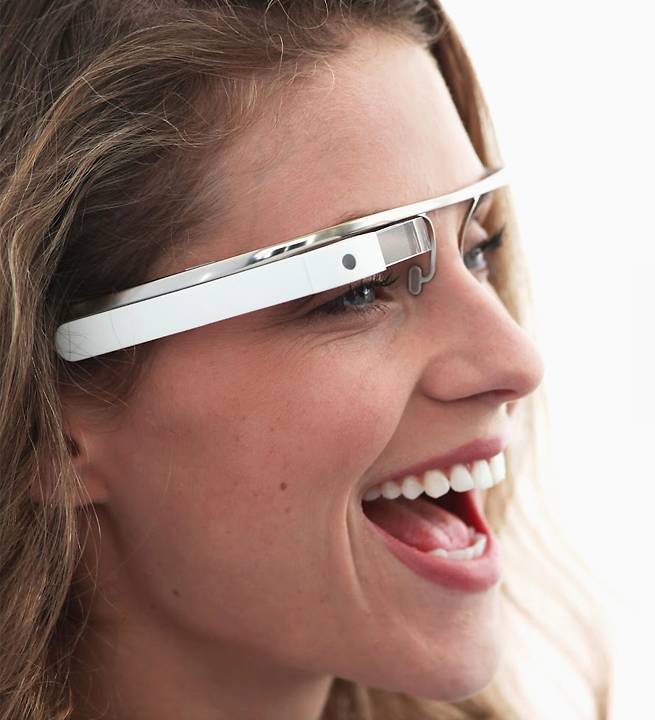
\includegraphics[height=.2\textheight]{img/google-glass.png}};
    \node [right=6em of user, visible on= <2->] (server) {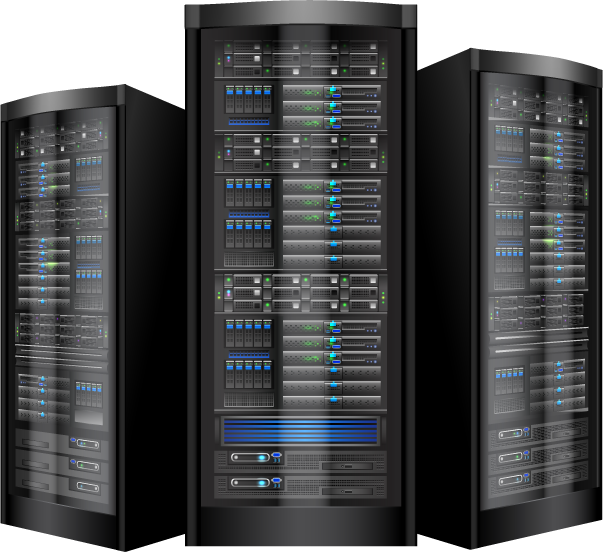
\includegraphics[height=.2\textheight]{img/server.png}};
    \path (user) -- coordinate[midway] (center) (server);

    % surrounding images
    \node[left=1em of user] (pokemon) {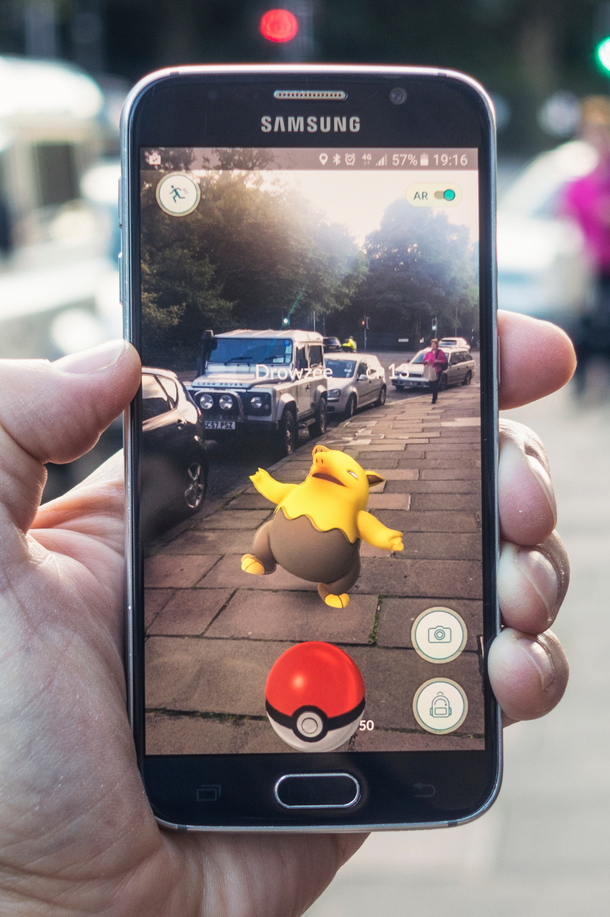
\includegraphics[height=.3\textwidth]{img/ar_pokemongo.jpg}};
    \node[right=1em of server] (ar) {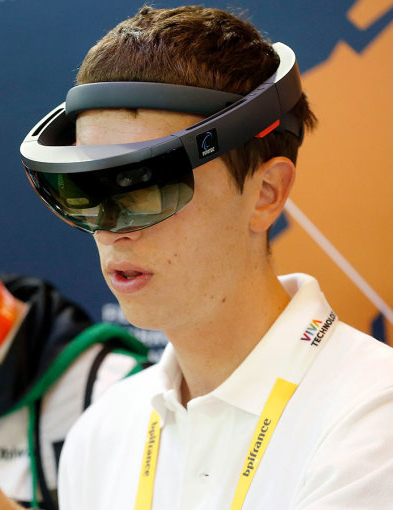
\includegraphics[height=.3\textwidth]{img/augmentedreality.jpg}};
    \node[above=5em of center] (hud) {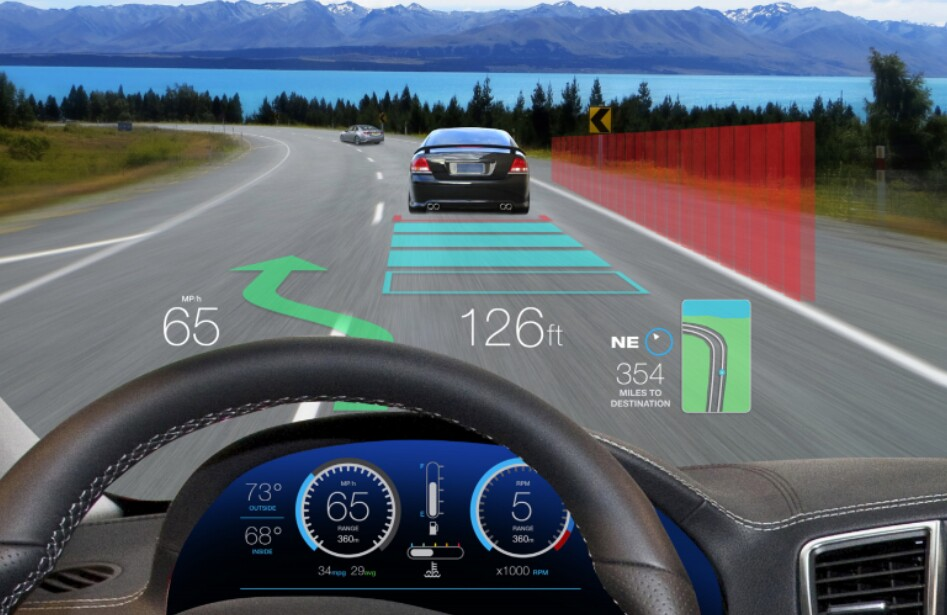
\includegraphics[height=.25\textheight]{img/AR_HUD_proc.jpg}};
    \node[below=7em of center] (glass) {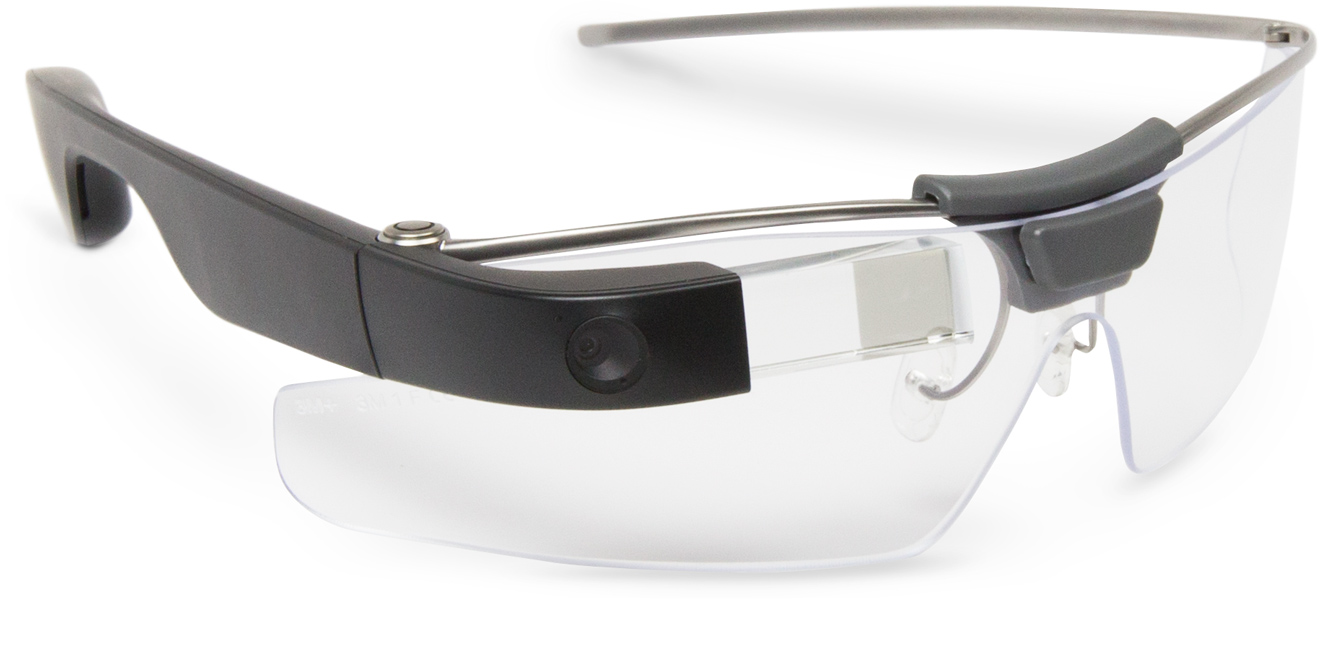
\includegraphics[height=.2\textheight]{img/glass_wearable.jpeg}};


    \path[draw, -{Latex[length=2mm]}, very thick, visible on= <2->]
    (user) edge [out=45, in=135] node[above] {Sensory Input} (server)
    (server) edge [out=225, in=315] node[below] {Human-parseable\\Feedback} (user);
\end{tikzpicture}